\documentclass{jarticle}
\usepackage[dvipdfmx]{graphicx}
\usepackage{here}


\begin{document}

\begin{titlepage}
\title{ユーザーズマニュアル}
\author{グループ15:1029289895 尾崎翔太、1029288619 山田宏暁}
\date{2018/6/15}

\maketitle
\end{titlepage}

\section{概要}
\hspace{10pt}SIMPLE/ext1は1語16ビットの簡単なコンピュータである。一方で、即値演算や関数呼び出しをサポートしており、プロセッサとして十分な機能を備えている。


\section{性能と特徴}
\subsection{性能}
\hspace{10pt}クロックの周波数は表1の通りである。
\begin{table}[htbp]
  \centering
  \caption{クロック周波数}
  \begin{tabular}{|c|c|} \hline
  クロック & 59.11MHz \\ \hline
  チャタリング防止用クロック & 164.02MHz \\ \hline
  \end{tabular}
\end{table}
これは、クリティカルパス(後述)を通る場合なので、そこを使わなければいくらか速くなる。また、LE数は3194である。

\subsection{特徴}
\begin{description}
\item[4フェーズの4段パイプライン] \leavevmode \\
1クロックで約1命令を実行できる。フォワーディングによりデータ・ハザードは起きない。
\item[スタック] \leavevmode \\
8KWのスタックを備えている。
\item[静的分岐予測] \leavevmode \\
分岐予測の方法は、プログラムの前方への分岐は失敗、後方への分岐は成功と予測する、というものである。失敗すればnop命令を挟む場合がある。
\item[即値演算] \leavevmode \\
加算と減算については即値演算をサポートしている。
\item[1命令分岐] \leavevmode \\
比較と分岐を1命令で実行できる。
\item[BAL/BR命令] \leavevmode \\
サブルーチン呼び出しのためのBAL命令(branch and link)とBR命令(branch register)をサポートしている。
\end{description}


\section{アーキテクチャ}
\subsection{メモリとレジスタ}
\hspace{10pt}SIMPLE/extは1語16ビットのコンピュータで、メモリやレジスタはいずれも16ビット幅である。また、ハーバード・アーキテクチャである。
\begin{itemize}
\item 命令メモリ \\
命令メモリのアドレスは12ビットであり、語単位にアドレスが付けられる。メモリの大きさは4KWである。
\item データメモリ \\
データメモリのアドレスは14ビットであり、語単位にアドレスが付けられる。メモリの大きさは16KWである。
\item スタック \\
スタックはスタックポップ/プッシュ命令で読み書きする。メモリの大きさは8KWである。
\item BAL/BR用スタック \\
BAL/BR命令で使用するスタックである。5個あり、大きさはそれぞれ256Wである。
\item 汎用レジスタ \\
8個の汎用レジスタが備えられ、演算のソース/デスティネーションやデータメモリのアドレス計算に用いられる。この内、4番レジスタ~7番レジスタはBAL/BR命令で退避/復元される。
\item プログラム・カウンタ \\
実行する命令のアドレスを保持する。BAL/BR命令で退避/復元される。
\end{itemize}


\subsection{命令セット・アーキテクチャ}
\hspace{10pt}SIMPLE/extの命令セット・アーキテクチャについて説明する。SIMPLE/extの命令形式を図1に示す。
\begin{figure}[htbp]
  \centering
  \caption{命令形式}
  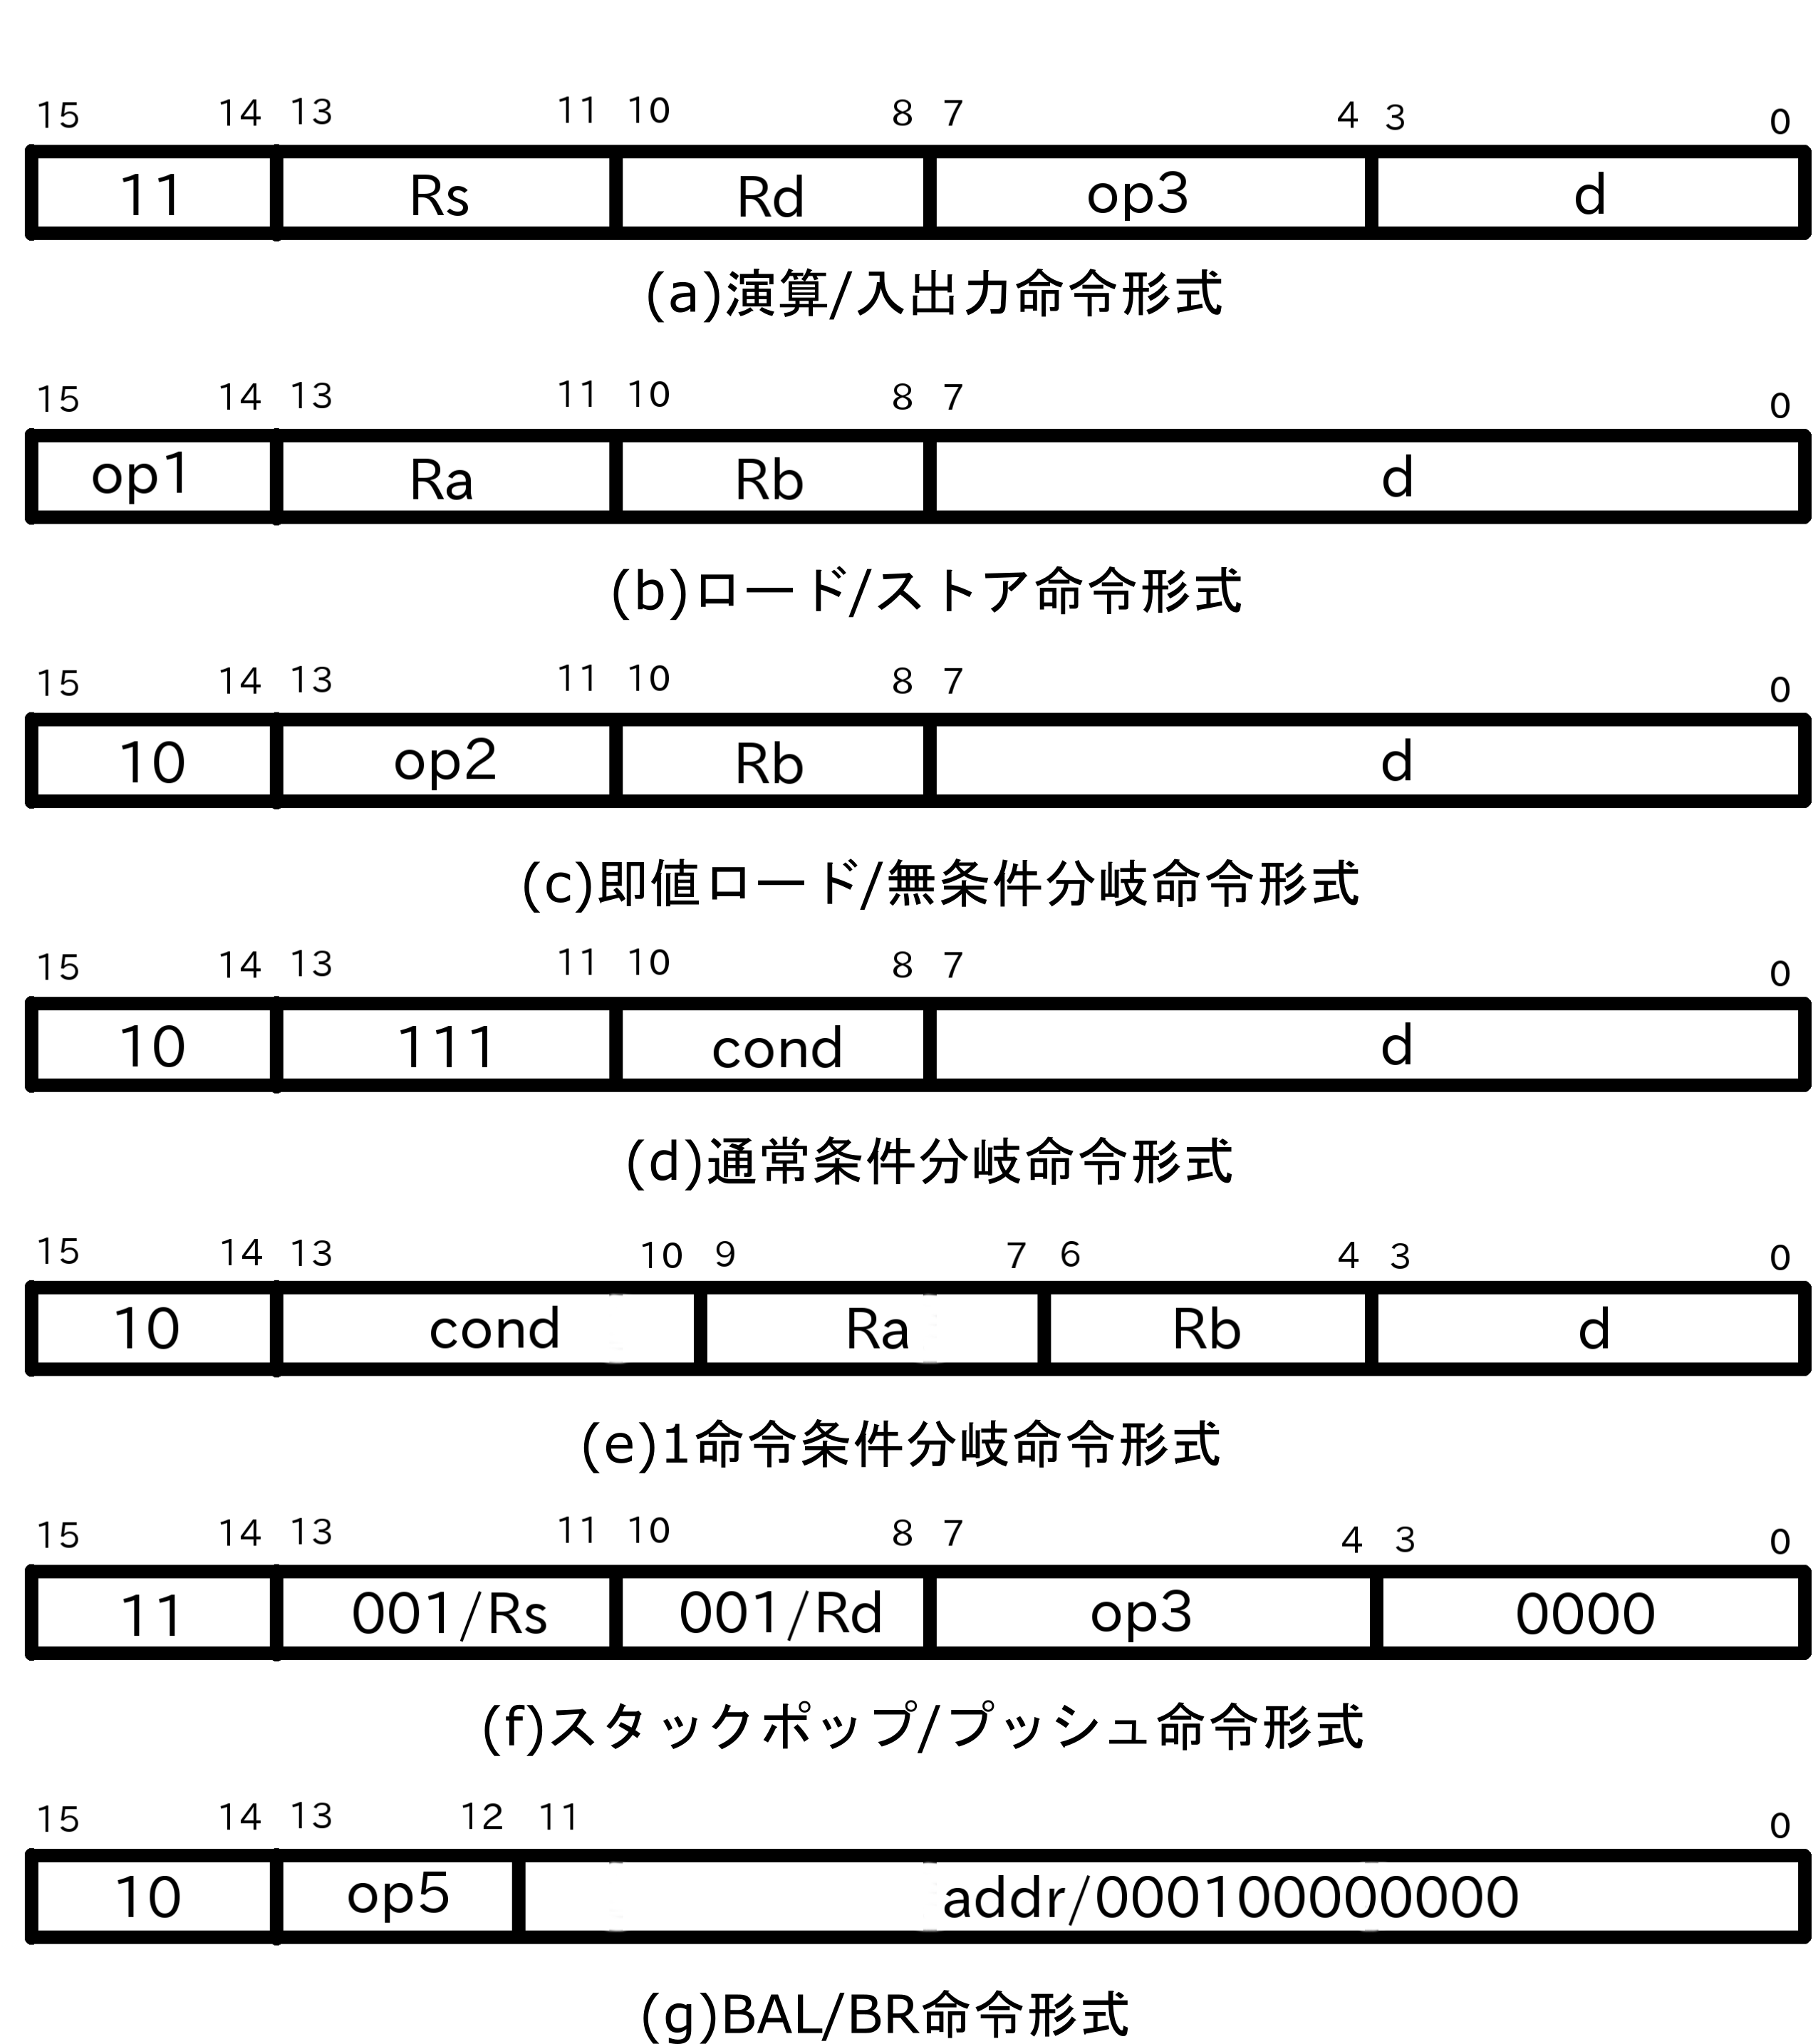
\includegraphics[width=\hsize]{instform.png}
\end{figure}
また、各命令についての説明で、Tableに載っていない操作コードなどを使用すると、他の命令が実行されたり、未定義の動作をしたりするので注意されたい。
\begin{description}
\item[命令形式] \leavevmode \\ 
命令はすべて1語(16ビット)の固定長であり、大きく7種類の形式がある。各命令形式とフィールドの意味は以下の通りである。
\begin{description}
\item[演算/入出力命令形式] \leavevmode \\
\begin{itemize}
\item $I_{15:14}$ (op1) ..... 操作コード (11)
\item $I_{13:11}$ (Rs) ..... ソース・レジスタ番号
\item $I_{10:8}$ (Rd) ..... デスティネーション・レジスタ番号
\item $I_{7:4}$ (op3) ..... 操作コード(0000 〜 1111)
\item $I_{3:0}$ (d) ..... シフト桁数/即値オペランド
\end{itemize}
\item[ロード/ストア形式] \leavevmode \\
\begin{itemize}
\item $I_{15:14}$ (op1) ..... 操作コード (00/01)
\item $I_{13:11}$ (Ra) ..... ソース/デスティネーションのレジスタ番号
\item $I_{10:8}$ (Rb) ..... ベース・レジスタ番号
\item $I_{7:0}$ (d) ..... 変位
\end{itemize}
\item[即値ロード/無条件分岐命令形式] \leavevmode \\
\begin{itemize}
\item $I_{15:14}$ (op1) ..... 操作コード (10)
\item $I_{13:11}$ (op2) ..... 操作コード (000 〜 110)
\item $I_{10:8}$ (Rb) ..... ソース/デスティネーション/ベースのレジスタ番号
\item $I_{7:0}$ (d) ..... 即値または変位
\end{itemize}
\item[通常条件分岐命令形式] \leavevmode \\
\begin{itemize}
\item $I_{15:14}$ (op1) ..... 操作コード (10)
\item $I_{13:11}$ (op2) ..... 操作コード (111)
\item $I_{10:8}$ (cond) ..... 分岐条件
\item $I_{7:0}$ (d) ..... 変位
\end{itemize}
\item[1命令条件分岐命令形式] \leavevmode \\
\begin{itemize}
\item $I_{15:14}$ (op1) ..... 操作コード (10)
\item $I_{13:10}$ (cond) ..... 分岐条件
\item $I_{9:7}$ (Ra) ..... 比較のオペランドとなるレジスタの番号
\item $I_{6:4}$ (Rb) ..... 比較のオペランドとなるレジスタの番号
\item $I_{3:0}$ (d) ..... 変位
\end{itemize}
\item[スタックポップ/プッシュ命令形式] \leavevmode \\
\begin{itemize}
\item $I_{15:14}$ (op1) ..... 操作コード (11)
\item $I_{13:11}$ (op2/Rs) ..... 操作コード (001) あるいは ソース・レジスタ番号
\item $I_{10:8}$ (op2/Rd) ..... 操作コード (001) あるいは デスティネーション・レジスタ番号
\item $I_{7:4}$ (op3) ..... 操作コード (1100/1101)
\item $I_{3:0}$ (op4) ..... 操作コード (0000)
\end{itemize}
\item[関数呼び出し命令形式] \leavevmode \\
\begin{itemize}
\item $I_{15:14}$ (op1) ..... 操作コード (10)
\item $I_{13:12}$ (op2) ..... 操作コード (01/10)
\item $I_{11:0}$ (address/op3) ..... ジャンプ先のアドレス あるいは 操作コード (000100000000)
\end{itemize}
\end{description}
\item[演算/入出力命令] \leavevmode \\
演算/入出力命令を表2に示す。演算命令では結果に基づく条件コードが出力される。
\begin{description}
\item[1.算術演算] \leavevmode \\
レジスタRdとRsの加算(ADD:add)、減算(SUB:subtract)または平均演算(AVG:average)の結果をRdに格納し、条件コードを設定する。また、加算と減算については、dフィールドが0でなく、Rsが000の場合、Rdとdの即値加算(ADDI:add immedeate)、即値減算(SUBI:substract immediate)となる。
\item[2.論理演算] \leavevmode \\
レジスタRdとRsのビット毎の論理積(AND:and)、論理和(OR:or)、または排他的論理和(XOR:exclusive-or)の結果をRdに格納し、条件コードを設定する。
\item[3.比較演算(CMP:compare)] \leavevmode \\
レジスタRdからRsを減算し、結果に基づく条件コードの設定のみを行う。
\item[4.移動演算(MOV:move)] \leavevmode \\
レジスタRdにRsの値を単に格納し、Rdの値に基づき条件コードを設定する。
\item[5.シフト演算] \leavevmode \\
レジスタRdの値を、以下のようにシフトした値をRdに格納し、条件コードを設定する。
\begin{itemize}
\item SLL (shift left logical) ..... 左論理シフト。左シフト後、空いた部分に0を入れる。
\item SLR (shift left rotate) ..... 左循環シフト。左シフト後、空いた部分にシフト・アウトされたビット列を入れる。
\item SRL (shift right logical) ..... 右論理シフト。右シフト後、空いた部分に0を入れる。
\item SRA (shift right arithmetic) ..... 右算術シフト。右シフト後、空いた部分に符号ビットの値を入れる。
\end{itemize}
シフト桁数は即値d(0〜15)である。条件コードVには常に0が設定される。
\item[6.入出力命令] \leavevmode \\
\begin{itemize}
\item IN(input) ..... スイッチなどの機器から入力した値をレジスタRdに格納する。
\item OUT(output) ..... レジスタRsの値を7SEG LEDなどの機器に出力する。
\item HLT(halt) ..... SIMPLE/extを停止させる。なお、後述するexecで停止状態を解除できる。
\end{itemize}
\end{description}
\begin{figure}[H]
  \centering
  \caption{演算/入出力命令形式}
  \includegraphics[width=0.66\hsize]{one.png}
\end{figure}
\begin{table}[H]
  \centering
  \caption{演算/入出力命令}
  \begin{tabular}{|c|c|l|} \hline
  mnemonic & op3 & function \\ \hline
  ADD\ Rd,Rs & 0000 & r[Rd]\ =\ r[Rd]\ +\ r[Rs] \\
  ADDI\ Rd, d & 0000 & r[Rd]\ =\ r[Rd]\ +\ d \\
  SUB\ Rd,Rs & 0001 & r[Rd]\ =\ r[Rd]\ -\ r[Rs] \\
  SUBI\ Rd, d & 0001 & r[Rd]\ =\ r[Rd]\ -\ d \\
  AND\ Rd,Rs & 0010 & r[Rd]\ =\ r[Rd]\ \&\ r[Rs] \\
  OR\ Rd,Rs & 0011 & r[Rd]\ =\ r[Rd]\ \textbar\  r[Rs] \\
  XOR\ Rd,Rs & 0100 & r[Rd]\ =\ r[Rd]\ \^\ r[Rs] \\
  CMP\ Rd,Rs & 0101 & r[Rd]\ -\ r[Rs] \\
  MOV\ Rd,Rs & 0110 & r[Rd]\ =\ r[Rs] \\
  AVG\ Rd,Rs & 0111 & r[Rd]\ =\ average(r[Rd], r[Rs]) \\
  SLL\ Rd,d & 1000 & r[Rd]\ =\ shift\_left\_logical(r[Rd],d) \\
  SLR\ Rd,d & 1001 & r[Rd]\ =\ shift\_left\_rotate(r[Rd],d) \\
  SRL\ Rd,d & 1010 & r[Rd]\ =\ shift\_right\_logical(r[Rd],d) \\
  SRA\ Rd,d & 1011 & r[Rd]\ =\ shift\_right\_arithmetic(r[Rd],d) \\
  IN\ Rd & 1100 & r[Rd]\ =\ input \\
  OUT\ Rs & 1101 & output\ =\ r[Rs] \\
  HLT & 1111 & halt() \\ \hline
  \end{tabular}
\end{table}
\item[ロード/ストア命令] \leavevmode \\
ロード命令(LD:load)とストア命令(store)は表3の通りである。ソース/デスティネーションは、フィールドRaで指定されたレジスタRaである。また実行アドレスはベース・レジスタ・アドレス指定により、フィールドRbで指定されたレジスタRbと、フィールドdを符号拡張したsign\_ext(d)を加算して求める。
\begin{figure}[H]
  \centering
  \caption{ロード/ストア命令形式}
  \includegraphics[width=0.66\hsize]{two.png}
\end{figure}
\begin{table}[H]
  \centering
  \caption{ロード/ストア命令}
  \begin{tabular}{|c|c|l|} \hline
  mnemonic & op1 & function \\ \hline
  LD\ Ra,d(Rb) & 00 & r[Ra]\ =\ *(r[Rb]\ +\ sign\_ext(d)) \\
  ST\ Ra,d(Rb) & 01 & *(r[Rb]\ +\ sign\_ext(d))\ =\ r[Ra] \\ \hline
  \end{tabular}
\end{table}
\item[即値ロード/無条件分岐命令] \leavevmode \\
即値ロード命令(LI:load immediate)と、上位8ビット即値ロード命令(ULI:upper load immediate)と、無条件分岐命令(B:branch)は表4の通りである。
\begin{itemize}
\item LI ..... 即値sign\_ext(d)をレジスタRbに格納する。
\item ULI ..... 即値dをレジスタRbの上位8ビットに格納する。下位8ビットには何もしない。
\item B ..... dを符号拡張した値を変位として、PC相対アドレス指定による分岐を行う。
\end{itemize}
\begin{figure}[H]
  \centering
  \caption{即値ロード/無条件分岐命令形式}
  \includegraphics[width=0.66\hsize]{three.png}
\end{figure}
\begin{table}[H]
  \centering
  \caption{即値ロード/無条件分岐命令}
  \begin{tabular}{|c|c|l|} \hline
  mnemonic & op2 & function \\ \hline
  LI\ Rb,d & 000 & r[Rb]\ =\ sign\_ext(d) \\
  ULI\ Rb,d & 001 & r[Rb][15:7]\ =\ d \\
  B\ d & 100 & PC\ =\ PC\ +\ 1\ +\ sign\_ext(d) \\ \hline
  \end{tabular}
\end{table}
\item[通常条件分岐命令] \leavevmode \\
通常条件分岐命令は表5の通りである。フィールドcondで定められる分岐条件が成り立てばPC相対アドレスによる分岐を行い、成り立たなければ単に次の命令に移行する。条件コードの意味は以下の通りである。
\begin{itemize}
\item S:負ならば1、そうでなければ0
\item Z:ゼロならば1、そうでなければ0
\item V:演算結果が符号付き16ビットで表せる範囲を超えた場合は1、そうでなければ0
\end{itemize}
各命令の分岐条件は以下の通りである。
\begin{itemize}
\item BE(branch on equal-to) ..... 条件コードZが1
\item BLT(branch on less-than) ..... 条件コードSとVのXOR(S \^\ V)が1
\item BLE(branch on less-thann or equal-to) ..... Zまたは(S \^\ V)が1
\item BNE(branch on not-equal-to) ..... 条件コードZが0
\end{itemize}
\begin{figure}[H]
  \centering
  \caption{通常条件分岐命令形式}
  \includegraphics[width=0.66\hsize]{four.png}
\end{figure}
\begin{table}[H]
  \centering
  \caption{通常条件分岐命令}
  \begin{tabular}{|c|c|l|} \hline
  mnemonic & cond & function \\ \hline
  BE\ d & 000 & if\ (Z)\ PC\ =\ PC\ +\ 1\ +\ sign\_ext(d) \\
  BLT\ d & 001 & if\ (S \^\ V)\ PC\ =\ PC\ +\ 1\ +\ sign\_ext(d) \\
  BLE\ d & 010 & if\ (Z \textbar\textbar \ (S \^\ V))\ PC\ =\ PC\ +\ 1\ +\  sign\_ext(d) \\
  BNE\ d & 011 & if\ (!Z)\ PC\ =\ PC\ +\ 1\ +\ sign\_ext(d) \\ \hline
  \end{tabular}
\end{table}
\item[1命令条件分岐命令] \leavevmode \\
1命令条件分岐命令はOBE(one instruction branch on equal-to)、OBLT(one instruction branch on less-than)、OBLE(one instruction branch on less-than or equal-to)、OBNE(one instructoin branch on not-equal-to)の4つで、表6の通りである。フィールドcondで定められる分岐条件が成り立てばPC相対アドレスによる分岐を行い、成り立たなければ単に次の命令に移行する。各命令はレジスタRa、Rbを比較して、それぞれ分岐条件が成り立てばPC相対アドレスによる分岐を行い、成り立たなければ単に次の命令に移行する。条件コードは用いないが、意味の上では分岐条件は通常条件分岐命令と同じである。
\begin{figure}[H]
  \centering
  \caption{1命令条件分岐命令形式}
  \includegraphics[width=0.66\hsize]{five.png}
\end{figure}
\begin{table}[H]
  \centering
  \caption{1命令条件分岐命令}
  \begin{tabular}{|c|c|l|} \hline
  mnemonic & cond & function \\ \hline
  OBE\ Ra,Rb,d & 1010 & if\ (r[Ra]\ ==\ r[Rb])\ PC\ =\ PC\ +\ 1\ +\ sign\_ext(d) \\
  OBLT\ Ra,Rb,d & 1011 & if\ (r[Ra]\ $<$\ r[Rb])\ PC\ =\ PC\ +\ 1\ +\ sign\_ext(d) \\
  OBLE\ Ra,Rb,d & 1100 & if\ (r[Ra]\ $<$=\ r[Rb])\ PC\ =\ PC\ +\ 1\ +\ sign\_ext(d) \\
  OBNE\ Ra,Rb,d & 1101 & if\ (r[Ra]\ !=\ r[Rb])\ PC\ =\ PC\ +\ 1\ +\ sign\_ext(d) \\ \hline
  \end{tabular}
\end{table}
\item[スタックポップ/プッシュ命令] \leavevmode \\
スタックポップ命令(POP:pop)とスタックプッシュ命令(PUSH:push)は表7の通りである。スタックプッシュ命令はレジスタRsをスタックにプッシュする。スタックポップ命令はレジスタRdにスタックからポップする。
\begin{figure}[H]
  \centering
  \caption{スタックポップ/プッシュ命令形式}
  \includegraphics[width=0.66\hsize]{six.png}
\end{figure}
\begin{table}[H]
  \centering
  \caption{スタックポップ/プッシュ命令}
  \begin{tabular}{|c|c|c|c|l|} \hline
  mnemonic & Rs & Rd & op3 & function \\ \hline
  POP\ Rd & 001 & Rd & 1100 & r[Rd]\ =\ stack.pop() \\
  PUSH\ Rs & Rs & 001 & 1101 & stack.push(r[Rs]) \\ \hline
  \end{tabular}
\end{table}
\item[BAL/BR命令] \leavevmode \\
BAL命令(bal:branch and link)とBR命令(br:branch register)は表8の通りである。BAL命令はPC+1と4番レジスタ~7番レジスタを専用のスタックに退避して指定されたアドレスをそのまま実効アドレスとして分岐する。BR命令はPCと4番レジスタ~7番レジスタを復元する。
\begin{figure}[H]
  \centering
  \caption{BAL/BR命令形式}
  \includegraphics[width=0.66\hsize]{seven.png}
\end{figure}
\begin{table}[H]
  \centering
  \caption{BAL/BR命令}
  \begin{tabular}{|c|c|c|l|} \hline
  mnemonic & op5 & addr & function \\ \hline
  BAL\ addr & 01 & addr & escape(PC(+\ 1), r[4], r[5], r[6], r[7]) \\ 
            &    &      & and PC\ =\ addr \\
  BR & 10 & 000100000000 & recover(PC, r[4], r[5], r[6], r[7]) \\ \hline
  \end{tabular}
\end{table}
\end{description}


\section{構造と動作}
\subsection{入出力}
\hspace{10pt}入力は以下の5つである。
\begin{itemize}
\item clock ..... 動作クロック。クロックの立ち上がりエッジに同期して各フェーズを活性化する。
\item clk\_ch ..... チャタリング防止のためのクロック。後述するexecはチャタリングを防ぐ必要があり、そのためのクロックである。
\item reset ..... リセット信号。負論理であり、0のときスイッチが押されたと認識する。resetが0になるとすべてのレジスタをクリアする。
\item exec ..... 起動/停止信号。負論理であり、0のときスイッチが押されたと認識する。SIMPLE/extが停止状態にあるときにexecが1から0に変化すると、SIMPLE/extは命令の実行を開始する。SIMPLE/extが実行状態にあるときにexecが1から0に変化すると、命令の実行を停止する。
\item exin ..... 外部入力。16ビットの信号で、IN命令が実行されたときに値が読み込まれる。
\end{itemize}
出力は以下の1つである。
\begin{itemize}
\item exout ..... 外部出力。16ビットの信号で、OUT命令が実行されたときに値が変化する。
\end{itemize}

\subsection{構造}
\subsubsection{ブロック図}
\hspace{10pt}ブロック図を図8に示す。
\begin{figure}[htbp]
  \centering
  \caption{ブロック図}
  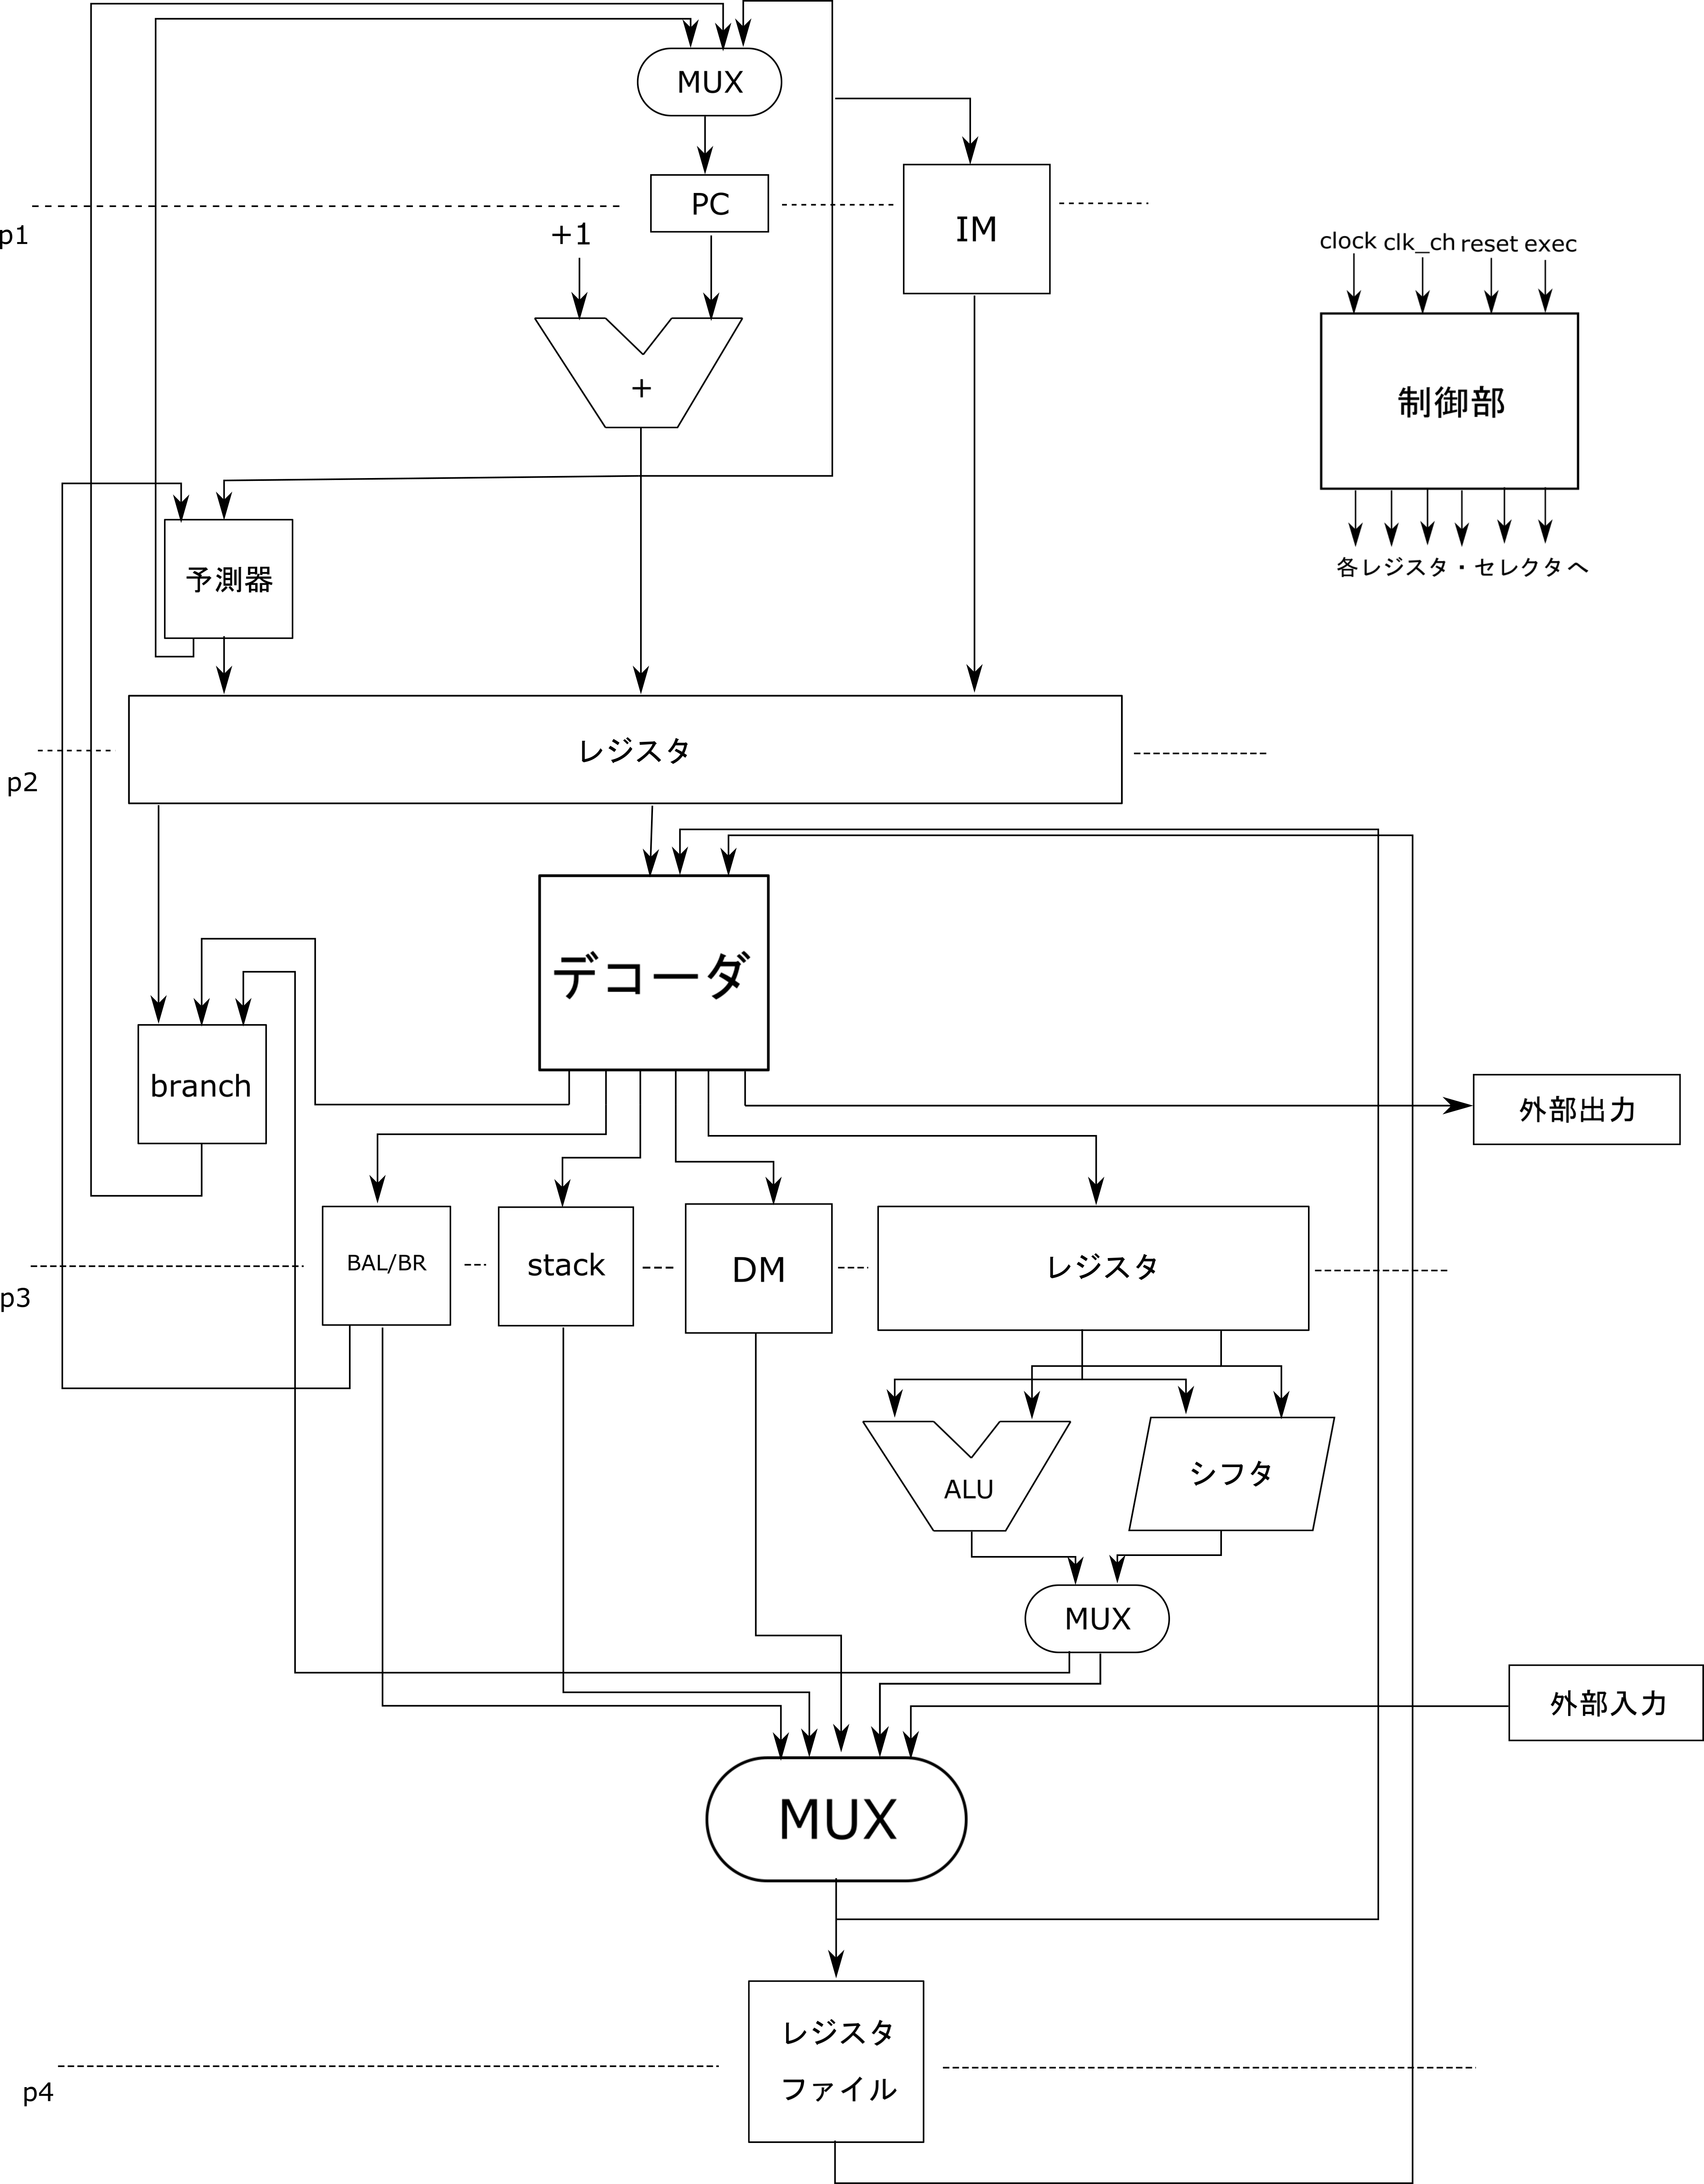
\includegraphics[width=\hsize]{block.png}
\end{figure}
実際にはexecの制御に関する回路やexoutの値を保つための回路などが存在するが、大まかには図8の通りである。
\subsubsection{フェーズ}
\hspace{10pt}SIMPLE/extはp1~p4の4フェーズで構成される。
\begin{description}
\item[p1(命令フェッチ/分岐予測)] \leavevmode \\
(分岐がなければ)PC+1のアドレスの命令を命令メモリからフェッチし、パイプラインレジスタに格納してPCの値をPC+1にする。またフェッチされた命令から分岐予測を行い分岐すると予測したならPCの値を書き換える。
\item[p2(デコード/レジスタ読み出し/アドレス計算/分岐確定)] \leavevmode \\
命令をデコードして様々な信号を送る。また、汎用レジスタから値を読みだして、命令に応じてパイプラインレジスタに格納する。命令がメモリアクセスの場合はアドレス計算も行う。さらに、フォワーディングもこのフェーズで行う。また、分岐を確定させるのもこのフェーズで、分岐予測が間違っていた場合はPCの値が適切になるように書き換える。
\item[p3(演算/メモリアクセス/スタックアクセス/BAL処理/BR処理/外部出力)] \leavevmode \\
演算やメモリアクセス等を行い、その結果を汎用レジスタの入力に置いておく。
\item[p4(レジスタ書き込み/外部入力)] \leavevmode \\
\end{description}

\end{document}
